\begin{figure}[ht]
    \centering
    \caption{Spatial Correlation Graphs of the Global Moran's I Index}
    \begin{subfigure}[b]{0.48\textwidth}
        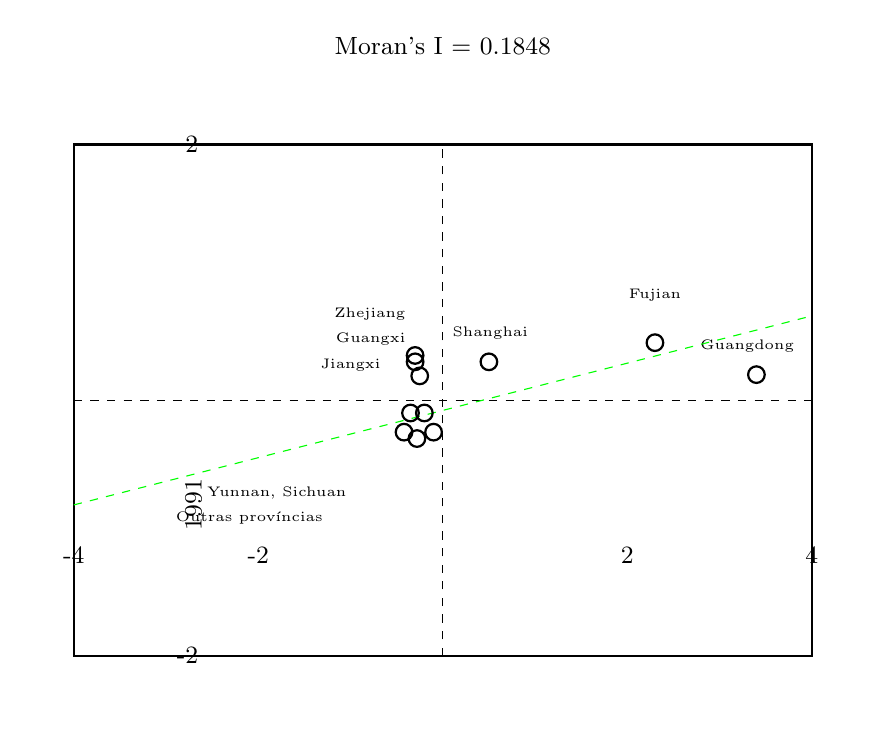
\begin{tikzpicture}
            \begin{axis}[
                width=\textwidth,
                height=0.8\textwidth,
                xmin=-4.5, xmax=4.5,
                ymin=-2.5, ymax=2.5,
                xtick={-4,-2,0,2,4},
                ytick={-2,0,2},
                xticklabels={-4,-2,0,2,4},
                yticklabels={-2,0,2},
                grid=none,
                axis lines=middle,
                xlabel={},
                ylabel={},
                title={Moran's I = 0.1848},
                title style={font=\small},
                axis line style={-},
                tick style={draw=none},
                ticklabel style={font=\small},
                axis on top=true,
                x axis line style={draw=none},
                y axis line style={draw=none},
                % Posicionamento dos ticks do eixo X (fora da moldura, abaixo)
                xtick style={draw=none, yshift=-2.5ex},
                x tick label style={
                    yshift=-3ex,
                    outer sep=35pt
                },
                % Posicionamento dos ticks do eixo Y (fora da moldura, esquerda)
                ytick style={draw=none, xshift=-2.5ex},
                y tick label style={
                    xshift=-3ex,
                    outer sep=70pt
                },
                % Ano vertical à esquerda
                extra y ticks={-2},
                extra y tick labels={1991},
                extra y tick style={
                    tick label style={rotate=90, anchor=west,xshift=-15pt, yshift=90pt, font=\small},
                    major tick length=0pt,
                    tickwidth=0pt
                }
            ]
                % Moldura quadrada
                \draw[black, thick] (axis cs:-4,-2) rectangle (axis cs:4,2);
                
                % Linhas de referência
                \addplot[dashed, black, no marks] coordinates {(-4,0) (4,0)};
                \addplot[dashed, black, no marks] coordinates {(0,-2) (0,2)};
                
                % Pontos das províncias (X991)
                \addplot[only marks, mark=o, mark options={scale=1.5, fill=white, line width=0.8pt}] coordinates {
                    (2.3,0.45) (0.5,0.3) (3.4,0.2) (-0.3,0.3) (-0.3,0.35) (-0.25,0.19)
                    (-0.2,-0.1) (-0.35,-0.1) (-0.28,-0.3) (-0.1,-0.25) (-0.42,-0.25)
                };
                
                % Rótulos
                \node[anchor=south, font=\fontsize{3}{3}\selectfont] at (2.3,0.7) {Fujian};
                \node[anchor=south west, font=\fontsize{3}{3}\selectfont] at (0.0,0.4) {Shanghai};
                \node[anchor=south, font=\fontsize{3}{3}\selectfont] at (3.3,0.3) {Guangdong};
                \node[anchor=north east, font=\fontsize{3}{3}\selectfont] at (-0.3,0.6) {Guangxi};
                \node[anchor=north east, font=\fontsize{3}{3}\selectfont] at (-0.3,0.8) {Zhejiang};
                \node[anchor=north, font=\fontsize{3}{3}\selectfont] at (-1, 0.4) {Jiangxi};
                \node[anchor=north west, font=\fontsize{3}{3}\selectfont] at (-3,-0.8) {Outras províncias};
                \node[anchor=north, font=\fontsize{3}{3}\selectfont] at (-1.8,-0.6) {Yunnan, Sichuan};
                
                % Linha de ajuste
                \addplot[green, dashed, domain=-4:4, samples=100] {0.1848*x - 0.08};
            \end{axis}
        \end{tikzpicture}
    \end{subfigure}
    \hfill
    \begin{subfigure}[b]{0.48\textwidth}
        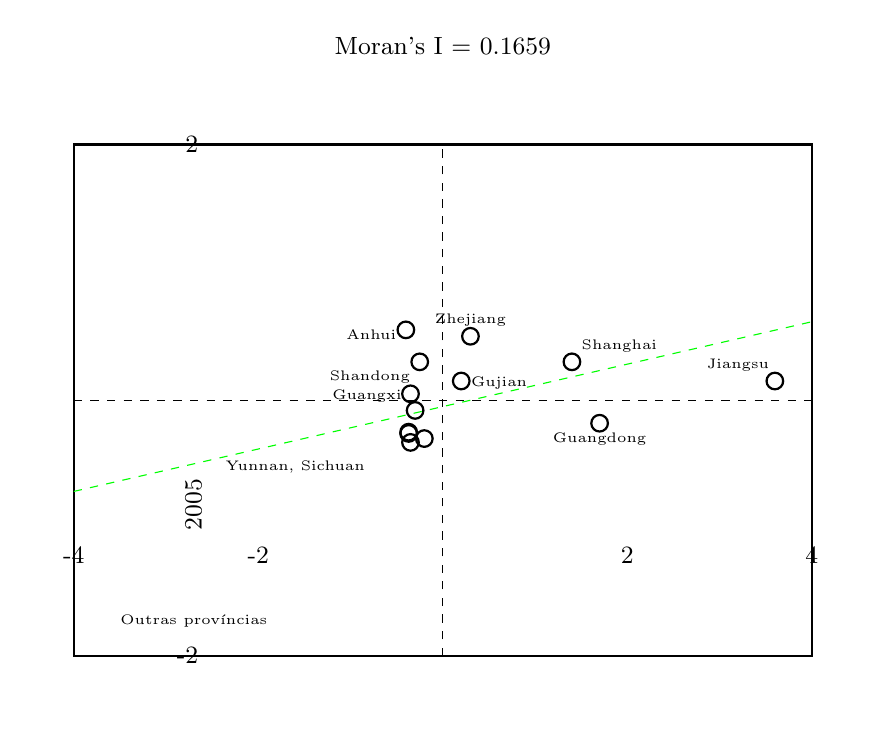
\begin{tikzpicture}
            \begin{axis}[
                width=\textwidth,
                height=0.8\textwidth,
                xmin=-4.5, xmax=4.5,
                ymin=-2.5, ymax=2.5,
                xtick={-4,-2,0,2,4},
                ytick={-2,0,2},
                xticklabels={-4,-2,0,2,4},
                yticklabels={-2,0,2},
                grid=none,
                axis lines=middle,
                xlabel={},
                ylabel={},
                title={Moran's I = 0.1659},
                title style={font=\small},
                axis line style={-},
                tick style={draw=none},
                ticklabel style={font=\small},
                axis on top=true,
                x axis line style={draw=none},
                y axis line style={draw=none},
                % Posicionamento dos ticks do eixo X (fora da moldura, abaixo)
                xtick style={draw=none, yshift=-2.5ex},
                x tick label style={
                    yshift=-3ex,
                    outer sep=35pt
                },
                % Posicionamento dos ticks do eixo Y (fora da moldura, esquerda)
                ytick style={draw=none, xshift=-2.5ex},
                y tick label style={
                    xshift=-3ex,
                    outer sep=70pt
                },
                % Ano vertical à esquerda
                extra y ticks={-2},
                extra y tick labels={2005},
                extra y tick style={
                    tick label style={rotate=90, anchor=west,xshift=-15pt, yshift=90pt, font=\small},
                    major tick length=0pt,
                    tickwidth=0pt
                }
            ]
                \draw[black, thick] (axis cs:-4,-2) rectangle (axis cs:4,2);
                
                % Linhas de referência
                \addplot[dashed, black, no marks] coordinates {(-4,0) (4,0)};
                \addplot[dashed, black, no marks] coordinates {(0,-2) (0,2)};
                
                % Pontos das províncias (X005)
                \addplot[only marks, mark=o, mark options={scale=1.5, fill=white, line width=0.8pt}] coordinates {
                    (3.6,0.15) (1.7,-0.18) (1.4,0.3) (0.2,0.15) (0.3,0.5) (-0.4,0.55)
                    (-0.25,0.3) (-0.35,0.05) (-0.30,-0.08) (-0.2,-0.30) (-0.35,-0.33)
                    (-0.37,-0.25) (-0.37,-0.26)
                };
                
                % Rótulos
                \node[anchor=south, font=\tiny] at (3.2,0.15) {Jiangsu};
                \node[anchor=north, font=\tiny] at (1.7,-0.18) {Guangdong};
                \node[anchor=south west, font=\tiny] at (1.4,0.3) {Shanghai};
                \node[anchor=south west, font=\tiny] at (0.2,0.01) {Gujian};
                \node[anchor=south, font=\tiny] at (0.3,0.5) {Zhejiang};
                \node[anchor=south east, font=\tiny] at (-0.4,0.4) {Anhui};
                \node[anchor=south east, font=\tiny] at (-0.25,0.06) {Shandong};
                \node[anchor=south east, font=\tiny] at (-0.34,-0.09) {Guangxi};
                \node[anchor=north, font=\fontsize{3}{3}\selectfont] at (-1.6,-0.4) {Yunnan, Sichuan};
                \node[anchor=north west, font=\tiny] at (-3.6,-1.6) {Outras províncias};
                
                % Linha de ajuste
                \addplot[green, dashed, domain=-4:4, samples=100] {0.1659*x - 0.05};
            \end{axis}
        \end{tikzpicture}
    \end{subfigure}
    
    \vspace{0.5cm}
    
    \begin{subfigure}[b]{0.48\textwidth}
        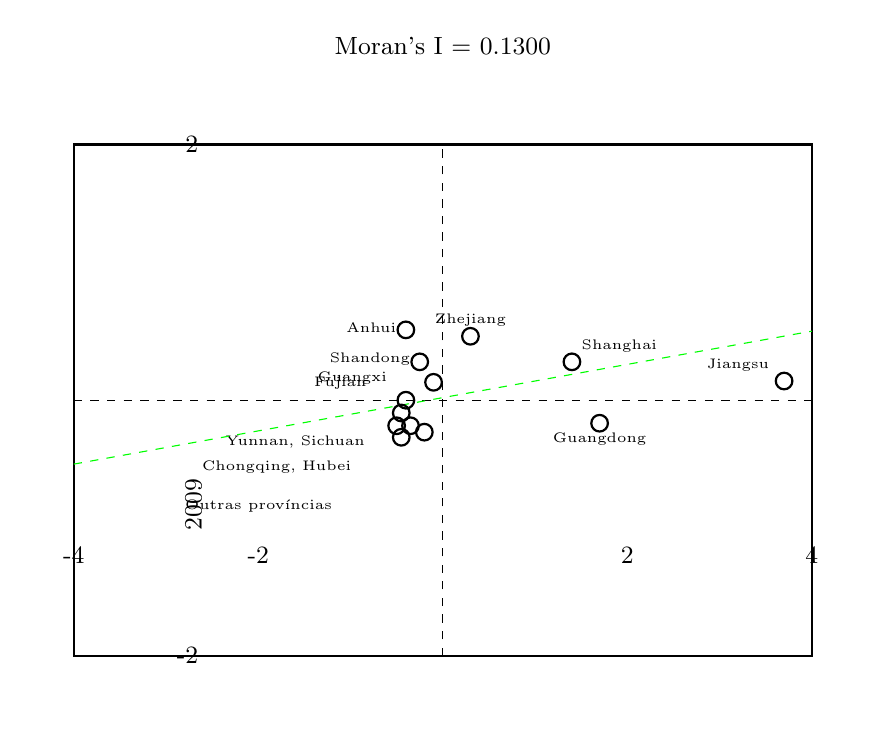
\begin{tikzpicture}
            \begin{axis}[
                width=\textwidth,
                height=0.8\textwidth,
                xmin=-4.5, xmax=4.5,
                ymin=-2.5, ymax=2.5,
                xtick={-4,-2,0,2,4},
                ytick={-2,0,2},
                xticklabels={-4,-2,0,2,4},
                yticklabels={-2,0,2},
                grid=none,
                axis lines=middle,
                xlabel={},
                ylabel={},
                title={Moran's I = 0.1300},
                title style={font=\small},
                axis line style={-},
                tick style={draw=none},
                ticklabel style={font=\small},
                axis on top=true,
                x axis line style={draw=none},
                y axis line style={draw=none},
                % Posicionamento dos ticks do eixo X (fora da moldura, abaixo)
                xtick style={draw=none, yshift=-2.5ex},
                x tick label style={
                    yshift=-3ex,
                    outer sep=35pt
                },
                % Posicionamento dos ticks do eixo Y (fora da moldura, esquerda)
                ytick style={draw=none, xshift=-2.5ex},
                y tick label style={
                    xshift=-3ex,
                    outer sep=70pt
                },
                % Ano vertical à esquerda
                extra y ticks={-2},
                extra y tick labels={2009},
                extra y tick style={
                    tick label style={rotate=90, anchor=west,xshift=-15pt, yshift=90pt, font=\small},
                    major tick length=0pt,
                    tickwidth=0pt
                }
            ]
                \draw[black, thick] (axis cs:-4,-2) rectangle (axis cs:4,2);
                
                % Linhas de referência
                \addplot[dashed, black, no marks] coordinates {(-4,0) (4,0)};
                \addplot[dashed, black, no marks] coordinates {(0,-2) (0,2)};
                
                % Pontos das províncias (X009)
                \addplot[only marks, mark=o, mark options={scale=1.5, fill=white, line width=0.8pt}] coordinates {
                    (3.7,0.15) (1.7,-0.18) (1.4,0.3) (0.3,0.5) (-0.4,0.55) (-0.25,0.3)
                    (-0.1,0.14) (-0.4,0) (-0.45,-0.1) (-0.35,-0.2) (-0.20,-0.25)
                    (-0.45,-0.29) (-0.50,-0.2)
                };
                
                % Rótulos
                \node[anchor=south, font=\tiny] at (3.2,0.15) {Jiangsu};
                \node[anchor=north, font=\tiny] at (1.7,-0.18) {Guangdong};
                \node[anchor=south west, font=\tiny] at (1.4,0.3) {Shanghai};
                \node[anchor=south, font=\tiny] at (0.3,0.5) {Zhejiang};
                \node[anchor=south east, font=\tiny] at (-0.4,0.45) {Anhui};
                \node[anchor=south east, font=\tiny] at (-0.25,0.2) {Shandong};
                \node[anchor=south west, font=\tiny] at (-1.5,0.01) {Fujian};
                \node[anchor=north east, font=\tiny] at (-0.5,0.3) {Guangxi};
                \node[anchor=north, font=\fontsize{3}{3}\selectfont] at (-1.6,-0.2) {Yunnan, Sichuan};
                 \node[anchor=north, font=\fontsize{3}{3}\selectfont] at (-1.8,-0.4) {Chongqing, Hubei};
                \node[anchor=north west, font=\tiny] at (-2.9,-0.7) {Outras províncias};
                
                % Linha de ajuste
                \addplot[green, dashed, domain=-4:4, samples=100] {0.1300*x + 0.02};
            \end{axis}
        \end{tikzpicture}
    \end{subfigure}
    \hfill
    \begin{subfigure}[b]{0.48\textwidth}
        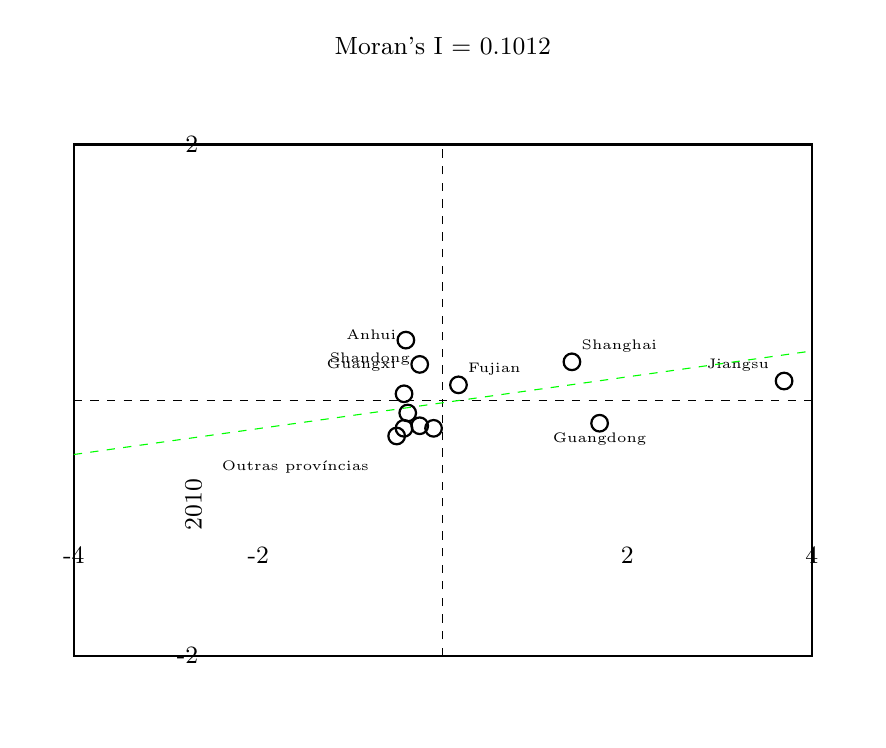
\begin{tikzpicture}
            \begin{axis}[
                width=\textwidth,
                height=0.8\textwidth,
                xmin=-4.5, xmax=4.5,
                ymin=-2.5, ymax=2.5,
                xtick={-4,-2,0,2,4},
                ytick={-2,0,2},
                xticklabels={-4,-2,0,2,4},
                yticklabels={-2,0,2},
                grid=none,
                axis lines=middle,
                xlabel={},
                ylabel={},
                title={Moran's I = 0.1012},
                title style={font=\small},
                axis line style={-},
                tick style={draw=none},
                ticklabel style={font=\small},
                axis on top=true,
                x axis line style={draw=none},
                y axis line style={draw=none},
                % Posicionamento dos ticks do eixo X (fora da moldura, abaixo)
                xtick style={draw=none, yshift=-2.5ex},
                x tick label style={
                    yshift=-3ex,
                    outer sep=35pt
                },
                % Posicionamento dos ticks do eixo Y (fora da moldura, esquerda)
                ytick style={draw=none, xshift=-2.5ex},
                y tick label style={
                    xshift=-3ex,
                    outer sep=70pt
                },
                % Ano vertical à esquerda
                extra y ticks={-2},
                extra y tick labels={2010},
                extra y tick style={
                    tick label style={rotate=90, anchor=west,xshift=-15pt, yshift=90pt, font=\small},
                    major tick length=0pt,
                    tickwidth=0pt
                }
            ]
                \draw[black, thick] (axis cs:-4,-2) rectangle (axis cs:4,2);
                
                % Linhas de referência
                \addplot[dashed, black, no marks] coordinates {(-4,0) (4,0)};
                \addplot[dashed, black, no marks] coordinates {(0,-2) (0,2)};
                
                % Pontos das províncias (X010)
                \addplot[only marks, mark=o, mark options={scale=1.5, fill=white, line width=0.8pt}] coordinates {
                    (3.7,0.15) (1.7,-0.18) (1.4,0.3) (0.17,0.12) (-0.4,0.47) (-0.25,0.28)
                    (-0.42,0.05) (-0.38,-0.1) (-0.42,-0.22) (-0.5,-0.28) (-0.25,-0.20)
                    (-0.1,-0.22)
                };
                
                % Rótulos
                \node[anchor=south, font=\tiny] at (3.2,0.15) {Jiangsu};
                \node[anchor=north, font=\tiny] at (1.7,-0.18) {Guangdong};
                \node[anchor=south west, font=\tiny] at (1.4,0.3) {Shanghai};
                \node[anchor=south west, font=\tiny] at (0.17,0.12) {Fujian};
                \node[anchor=south east, font=\tiny] at (-0.4,0.40) {Anhui};
                \node[anchor=south east, font=\tiny] at (-0.25,0.20) {Shandong};
                \node[anchor=north east, font=\tiny] at (-0.4,0.4) {Guangxi};
                \node[anchor=north west, font=\tiny] at (-2.5,-0.4) {Outras províncias};
                
                % Linha de ajuste
                \addplot[green, dashed, domain=-4:4, samples=100] {0.1012*x - 0.02};
            \end{axis}
        \end{tikzpicture}
    \end{subfigure}
    
  
    \caption*{Moran scatterplots illustrating the spatial autocorrelation among Chinese provinces across different years. Each dot represents a province, with labels strategically positioned for maximum readability. The dashed green line depicts the fitted linear relationship.}
    \caption*{Source: Compiled by the author.}
    \label{fig:moran_scatter}
\end{figure}
